% !TeX encoding = UTF-8
\section{Anhang}

%\myNewSection
%\begin{figure}[h]
%    \centering
%    
\includegraphics[width=0.7\textwidth]{res/IMG_A9A2347E0F7D-1.jpeg} 
%    \caption{iOS Schieberegler} 
%    \label{pic:schieberegler}
%\end{figure}
%\myNewSection
%\textbf{Stichpunkte:} 
%Ermüdende Informationsberge sollten in einen Anhang verbannt werden. (Wichtige Begriffe definieren)

%Beispiel: passende Lösung für dieses Problem zu finden
%\myNewSection \label{anhang:einleitung:passendeLösung}
%Um diese Idee \dq Stärken des Pc's sowie des Handys zu nutzen\dq noch etwas verständlicher zu machen, folgt eine kurzes Beispiel, wie diese Idee zu einem erfolgreichen Produkt geführt hat.
%Der erste Ipod\cite{einleitung_ipod} wurde 2001 vorgestellt und als \glqq tragbarer digitaler Medienabspielgeräte\grqq{} entworfen. Der Kleinheit und Portabilität zugunsten wurden nur die für das Gerät passenden und nötigen Funktionen implementiert. So zum Beispiel das Abspielen und Auswählen von Musik. Funktionen welche auf solch einem kleinen Gerät nicht gut funktionieren, wurden auf den Pc verlagert. So war der Pc für eine seiner Stärken zuständig, und zwar der Konfiguration, also dem Hinzufügen, Bearbeiten und Löschen von Musik. 

Link zum Repository: \url{https://git.imp.fu-berlin.de/thob97/bachelor-cli_calendar_app}
\newline
Commit-Hath: ab2bf74a810a521c61af575b9af284b2dc07eca0

\newpage
\myNewSection
%Appleiste
\begin{figure}
    \centering
    
\includegraphics[width=0.5\textwidth]{res/appbar_old.png} 
    \caption{Erstes Appleisten Design} 
    \label{pic:appleiste_old}
\end{figure}
\begin{figure}
    \centering
    
\includegraphics[width=0.5\textwidth]{res/appbar_new_home.png} 
    \caption{Aktuelles Appleisten Design} 
    \label{pic:appleiste_new}
\end{figure}

%Calendar
\begin{figure}
\centering
\begin{minipage}{.5\textwidth}
  \centering
  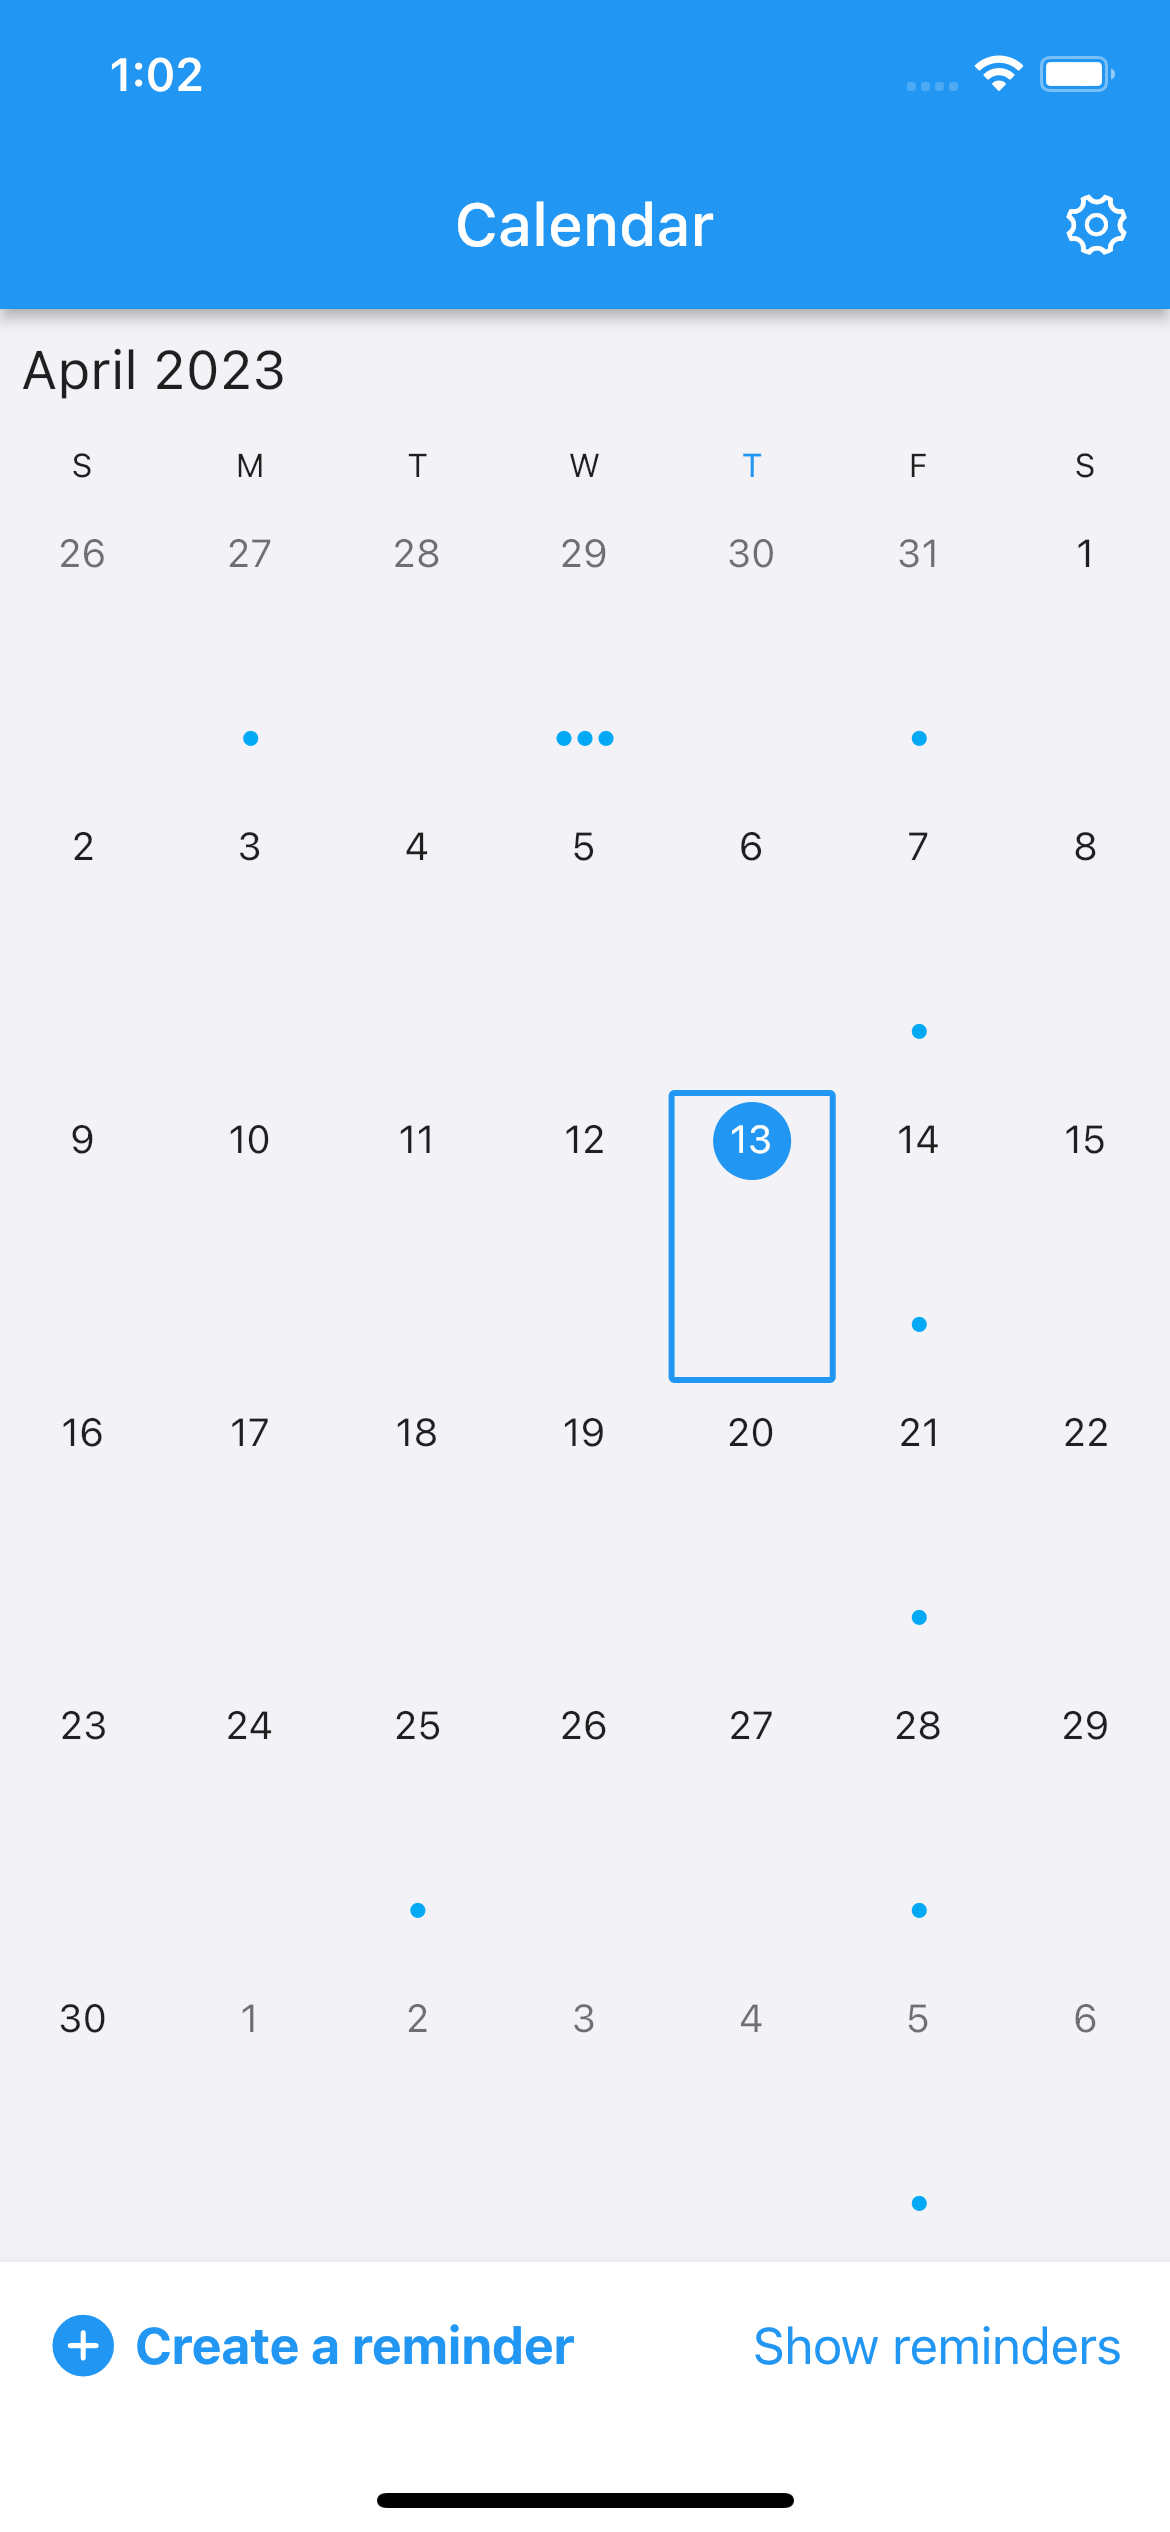
\includegraphics[width=0.8\linewidth]{res/calendar_view1.png}
  \captionof{figure}{Monatsansicht}
  \label{fig:calendar_view1}
\end{minipage}%
\begin{minipage}{.5\textwidth}
  \centering
  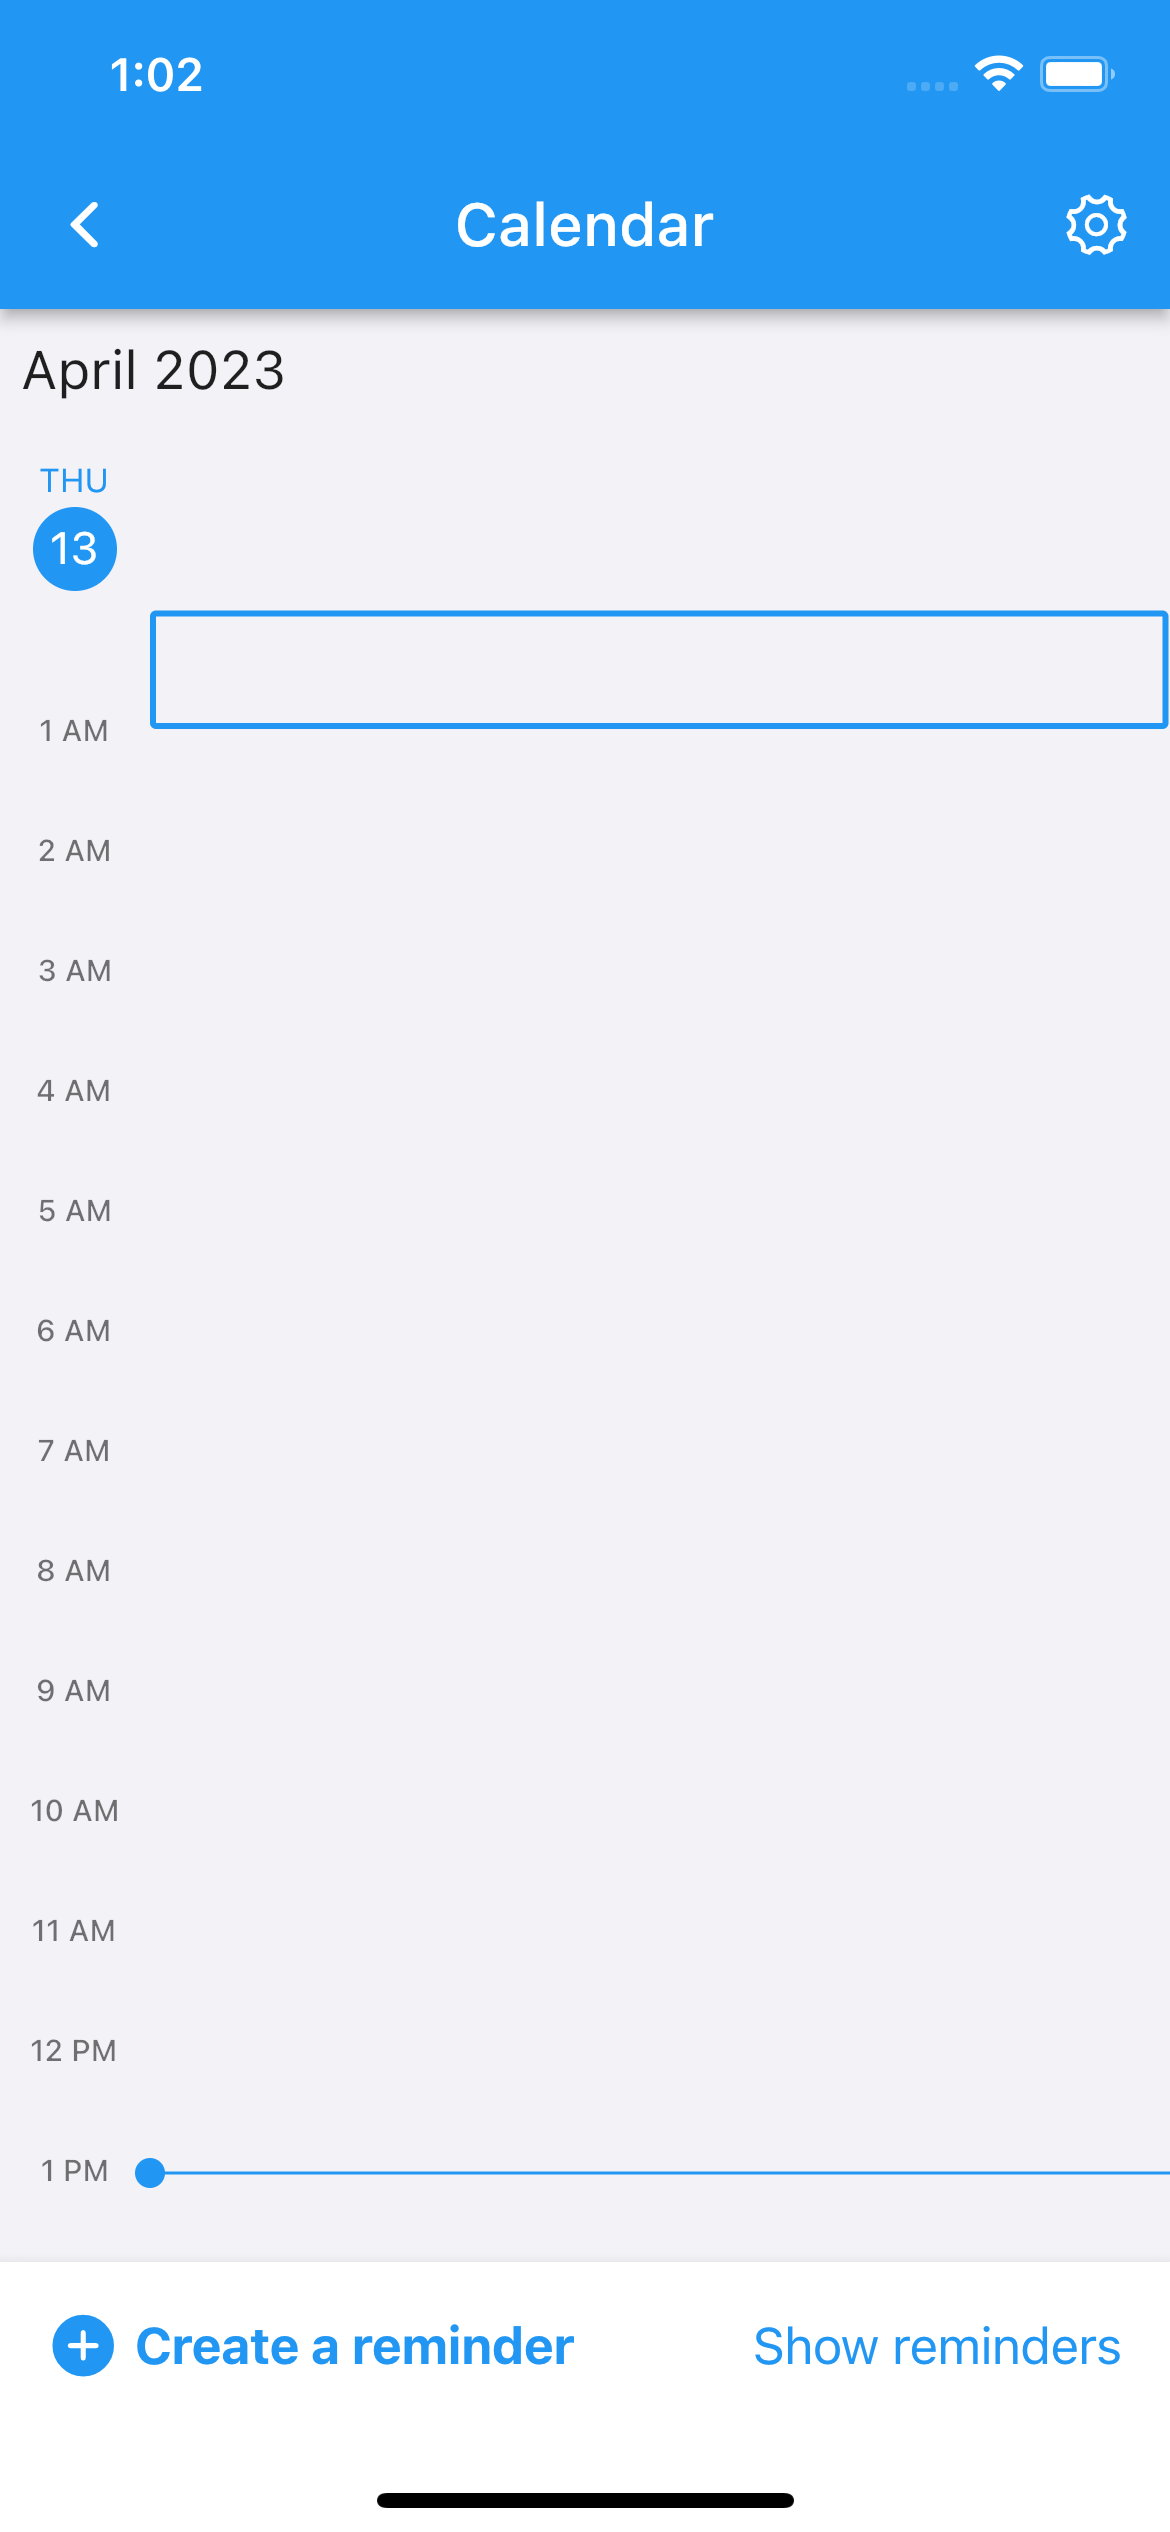
\includegraphics[width=0.8\linewidth]{res/calendar_view2.png}
  \captionof{figure}{Tagesansicht}
  \label{fig:calendar_view2}
\end{minipage}%
\end{figure}

%Reminder Page
\begin{figure}
    \centering
    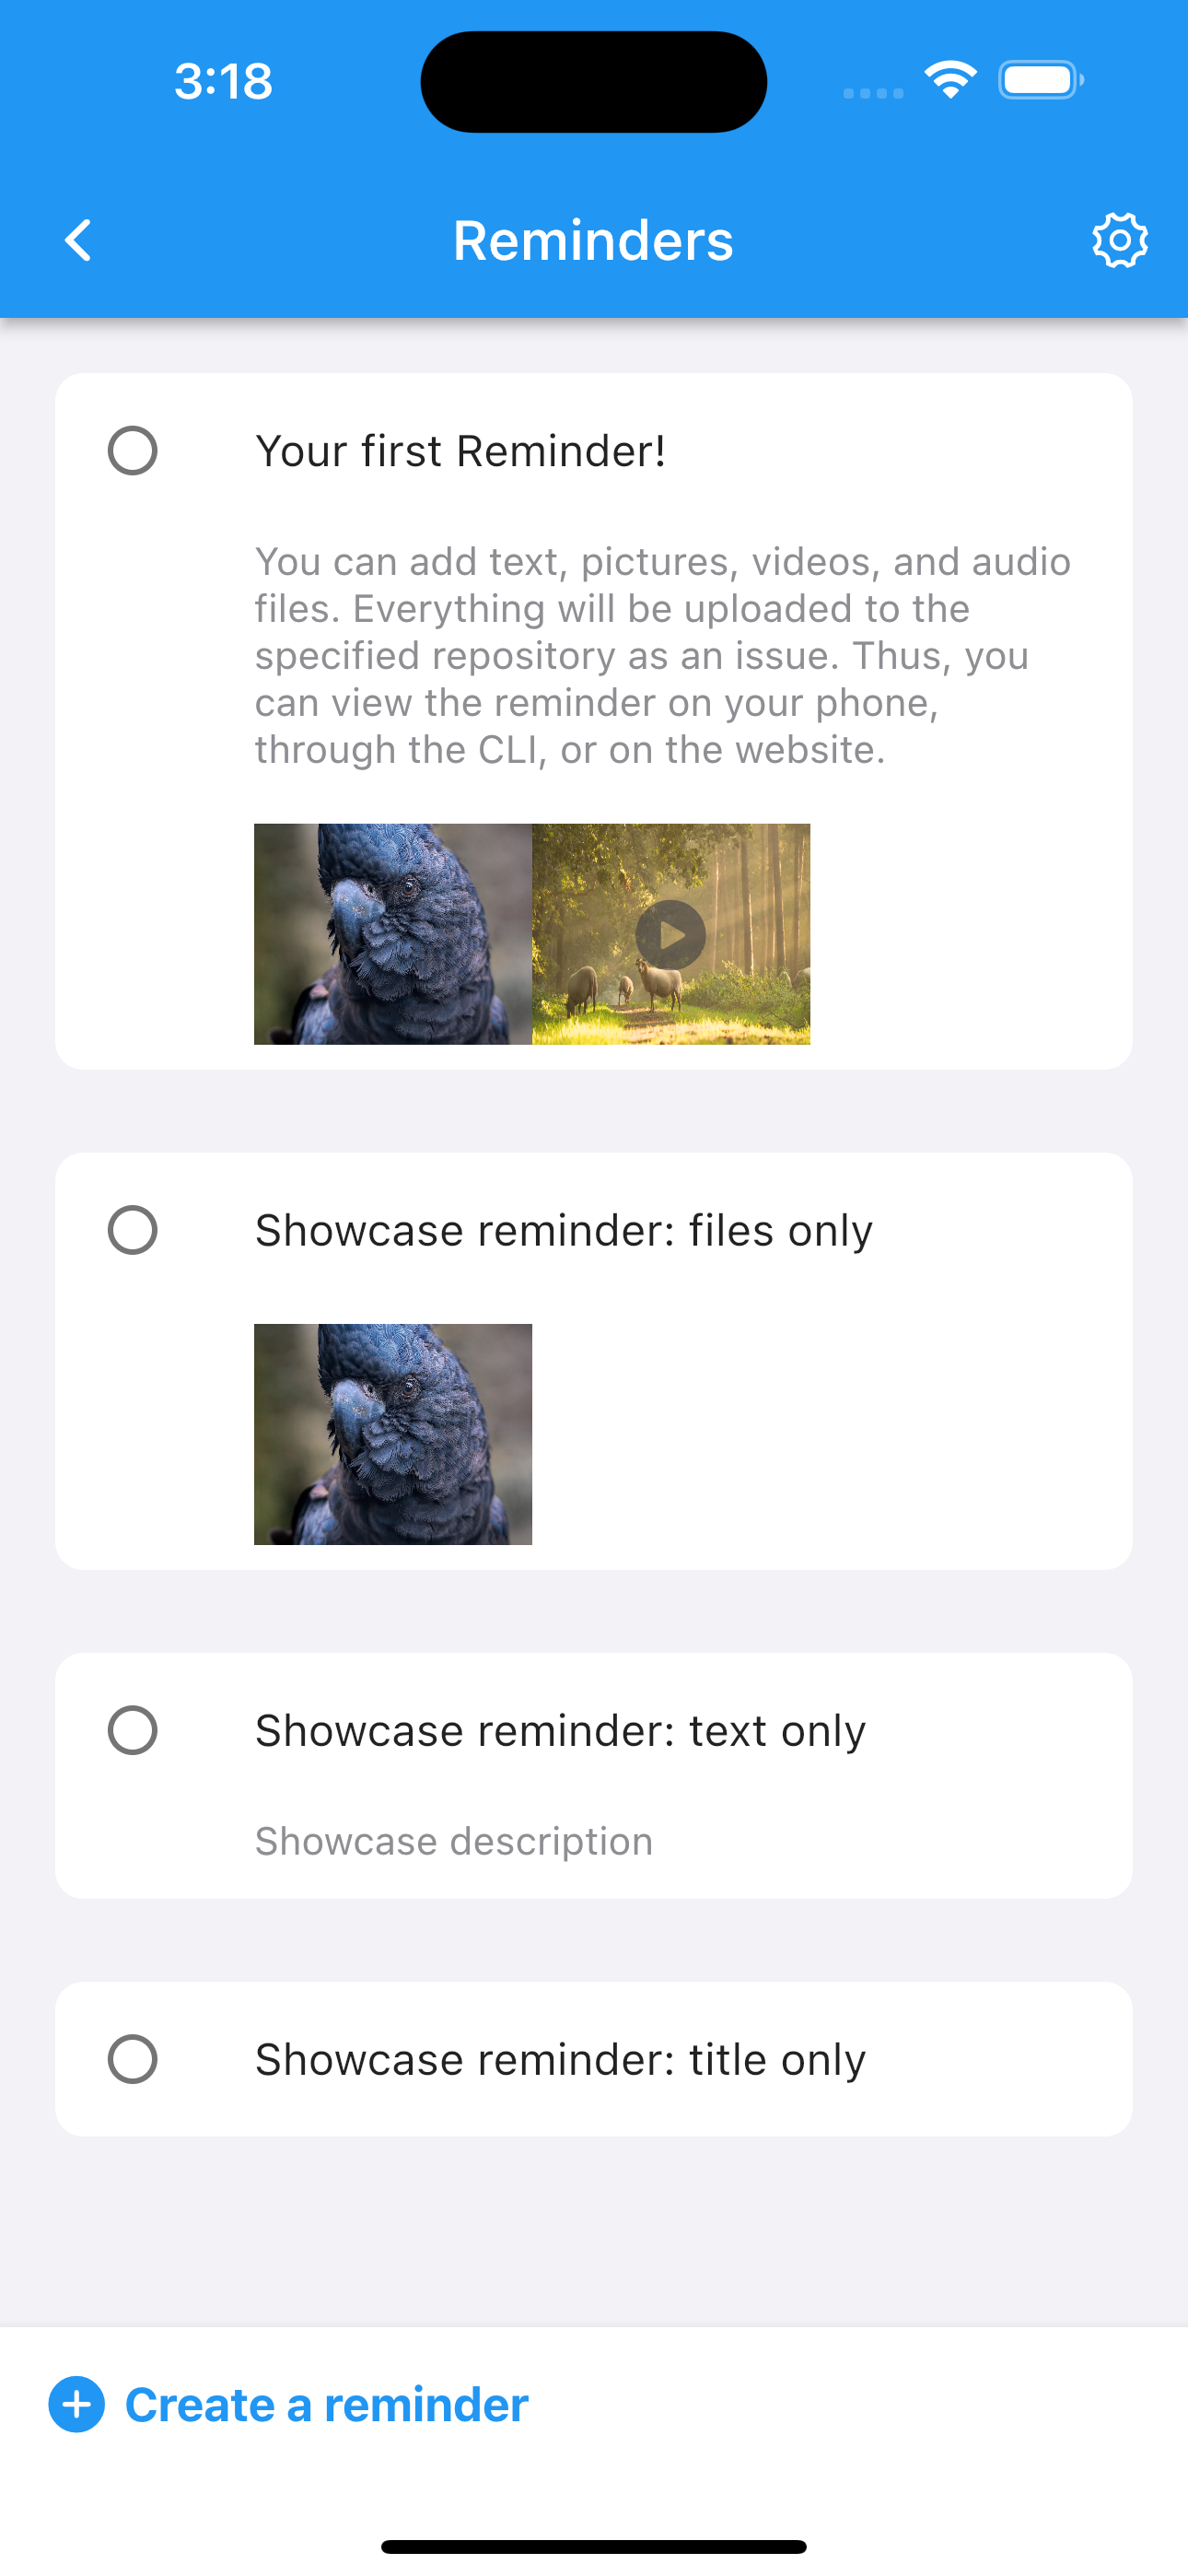
\includegraphics[width=0.5\textwidth]{res/reminders_page.png} 
    \caption{Erinnerungsseite mit Beispiel Erinnerungen} 
    \label{pic:reminders_page}
\end{figure}


%Settings
\begin{figure}
\centering
\begin{minipage}{.5\textwidth}
  \centering
  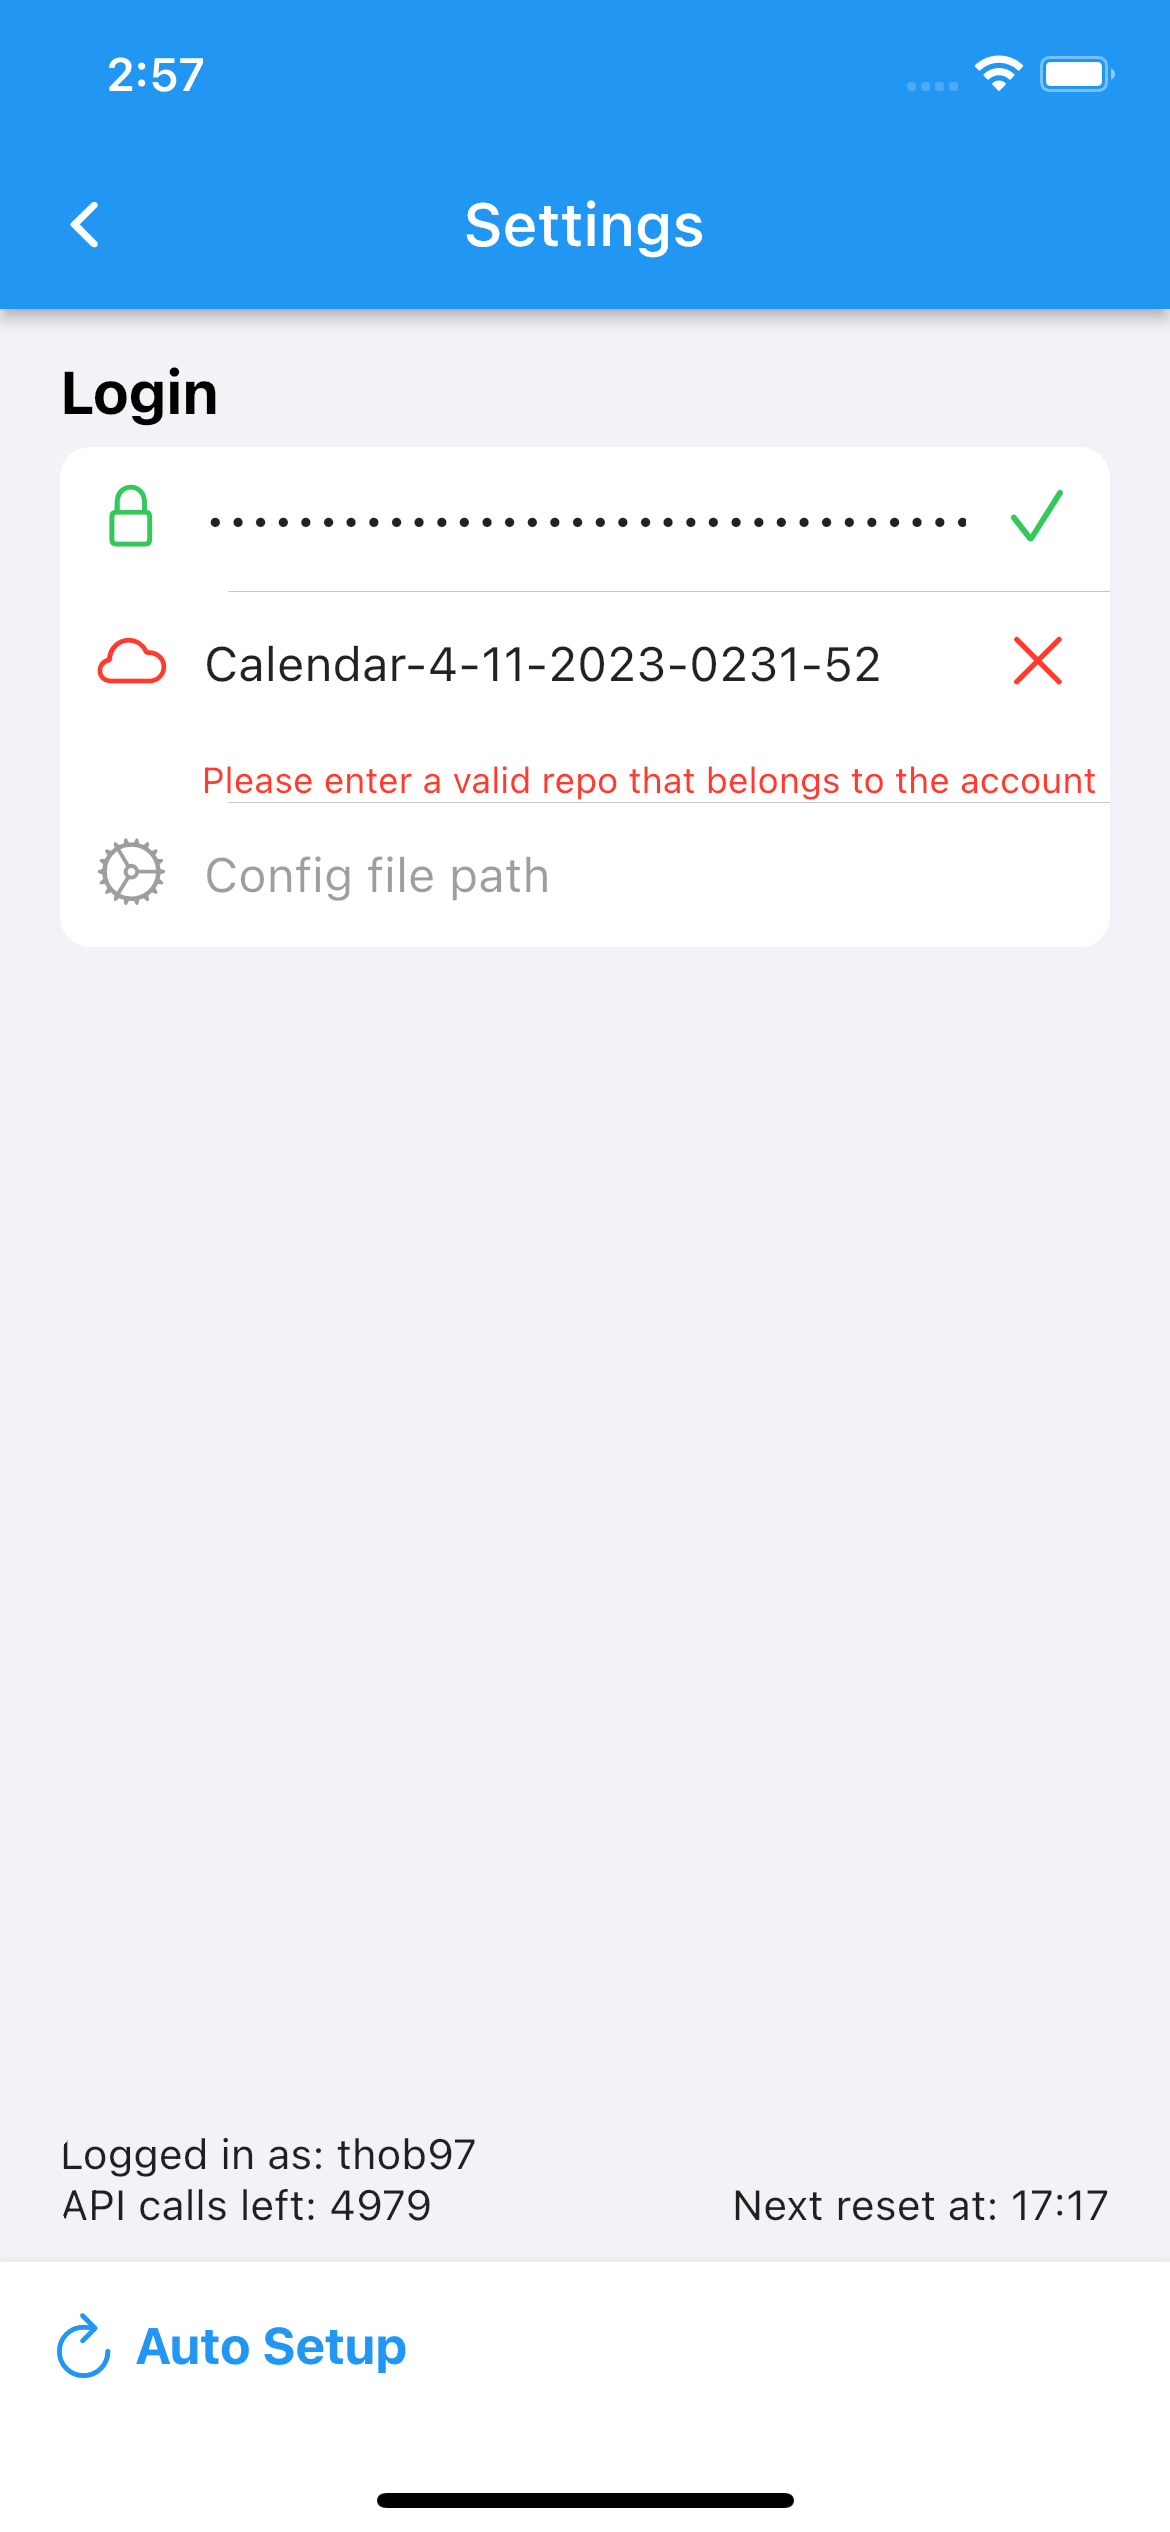
\includegraphics[width=0.9\linewidth]{res/settings_page.png}
  \captionof{figure}{Loginseite}
  \label{fig:settings_page}
\end{minipage}%
\begin{minipage}{.5\textwidth}
  \centering
  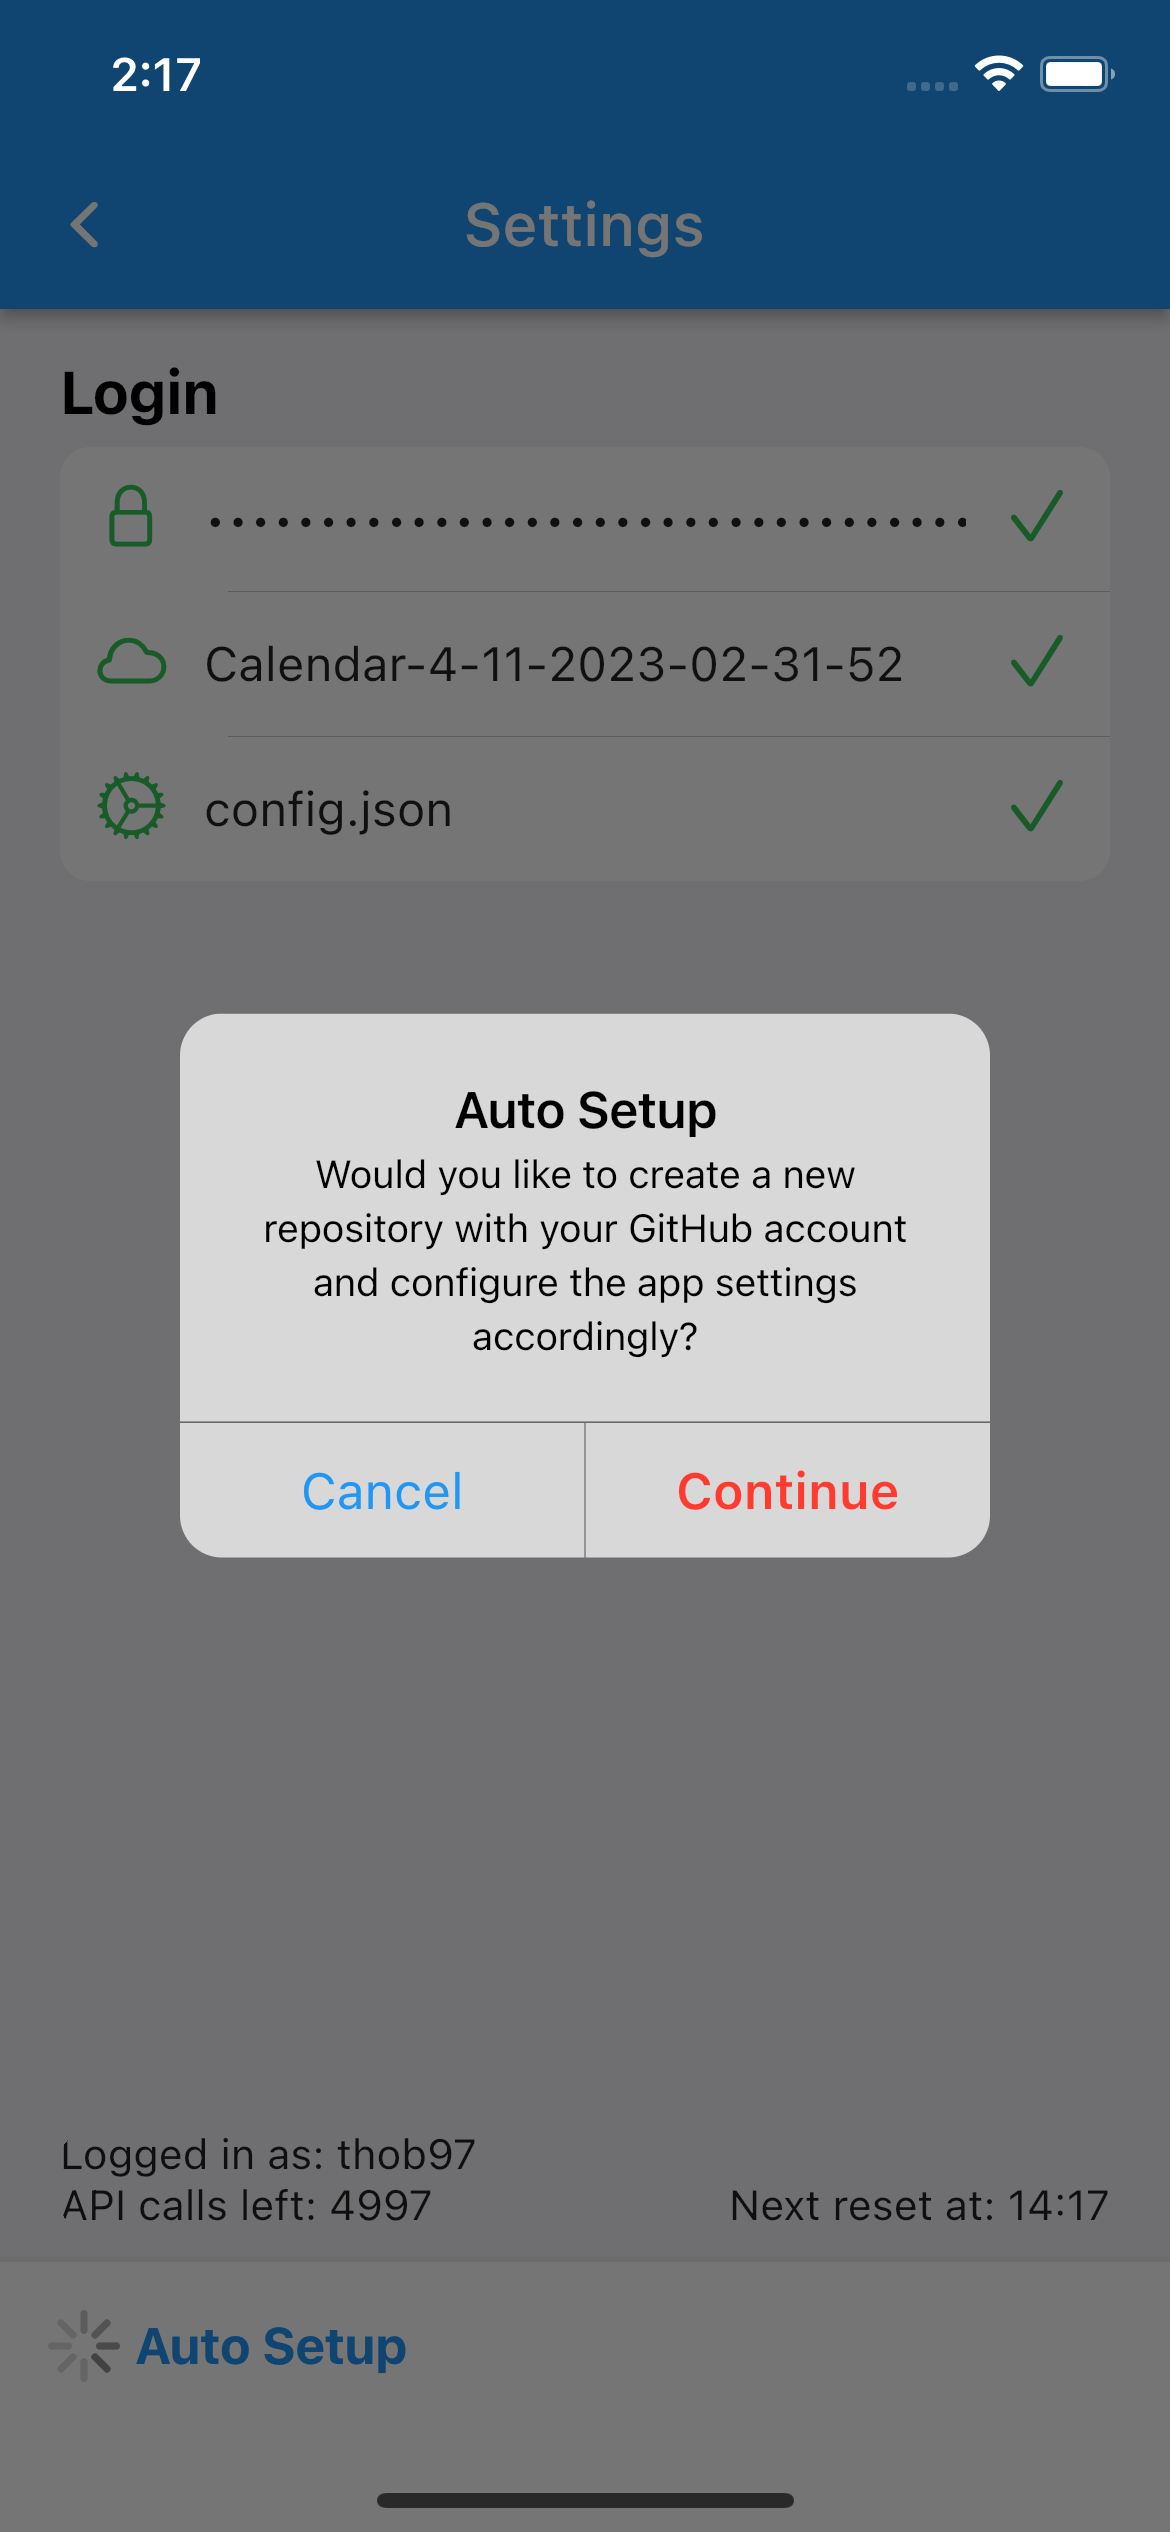
\includegraphics[width=0.9\linewidth]{res/settings_page_alert.png}
  \captionof{figure}{AutoSetup Alert}
  \label{fig:settings_page_alert}
\end{minipage}%
\end{figure}

%tastatur
\begin{figure}
    \centering
    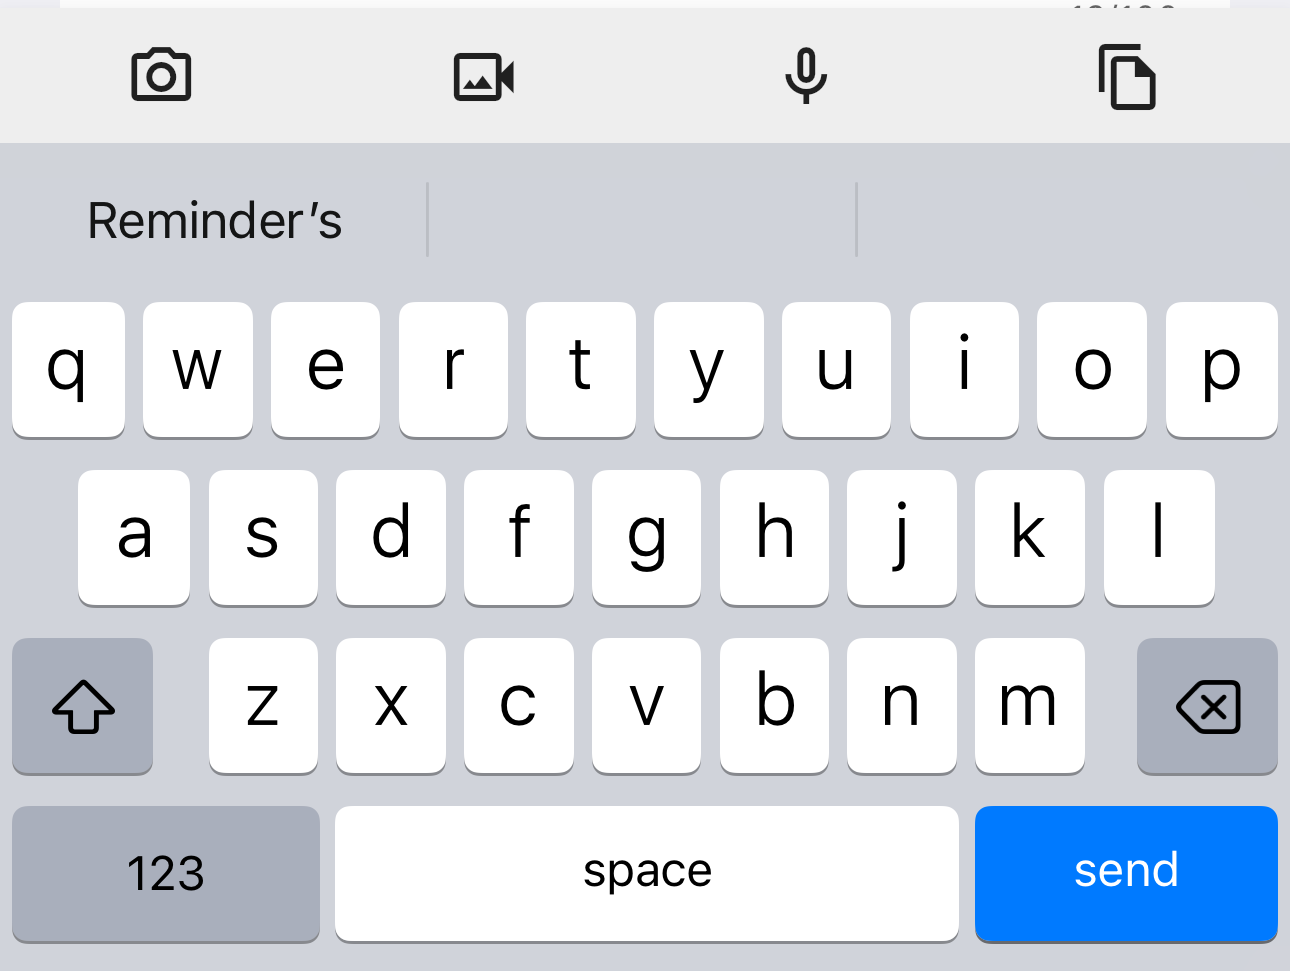
\includegraphics[width=0.6\textwidth]{res/tastatur.png} 
    \caption{Systemtastatur mit Icons} 
    \label{pic:tastatur}
\end{figure}

%WhenDate
\begin{figure}
    \centering
    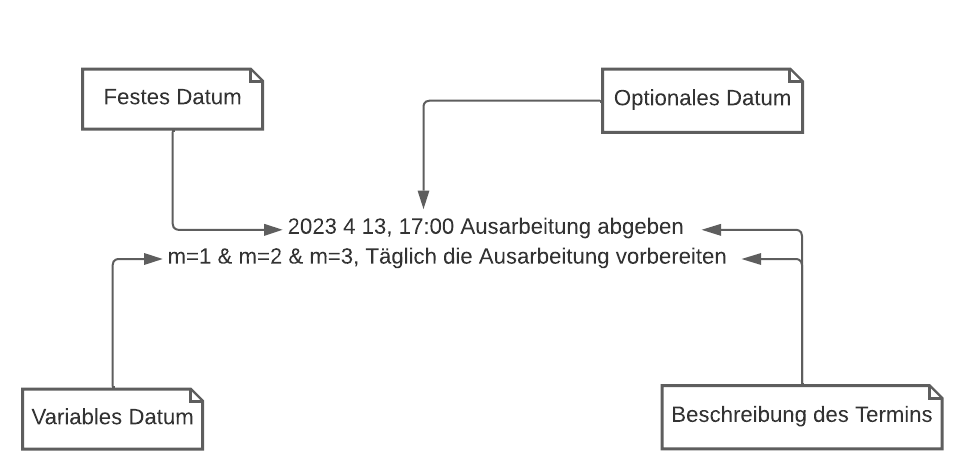
\includegraphics[width=0.9\textwidth]{res/when_termin.png} 
    \caption{Modellierter WhenTermin} 
    \label{pic:when_termin}
\end{figure}

%Zeitspanne
\begin{figure}
    \centering
    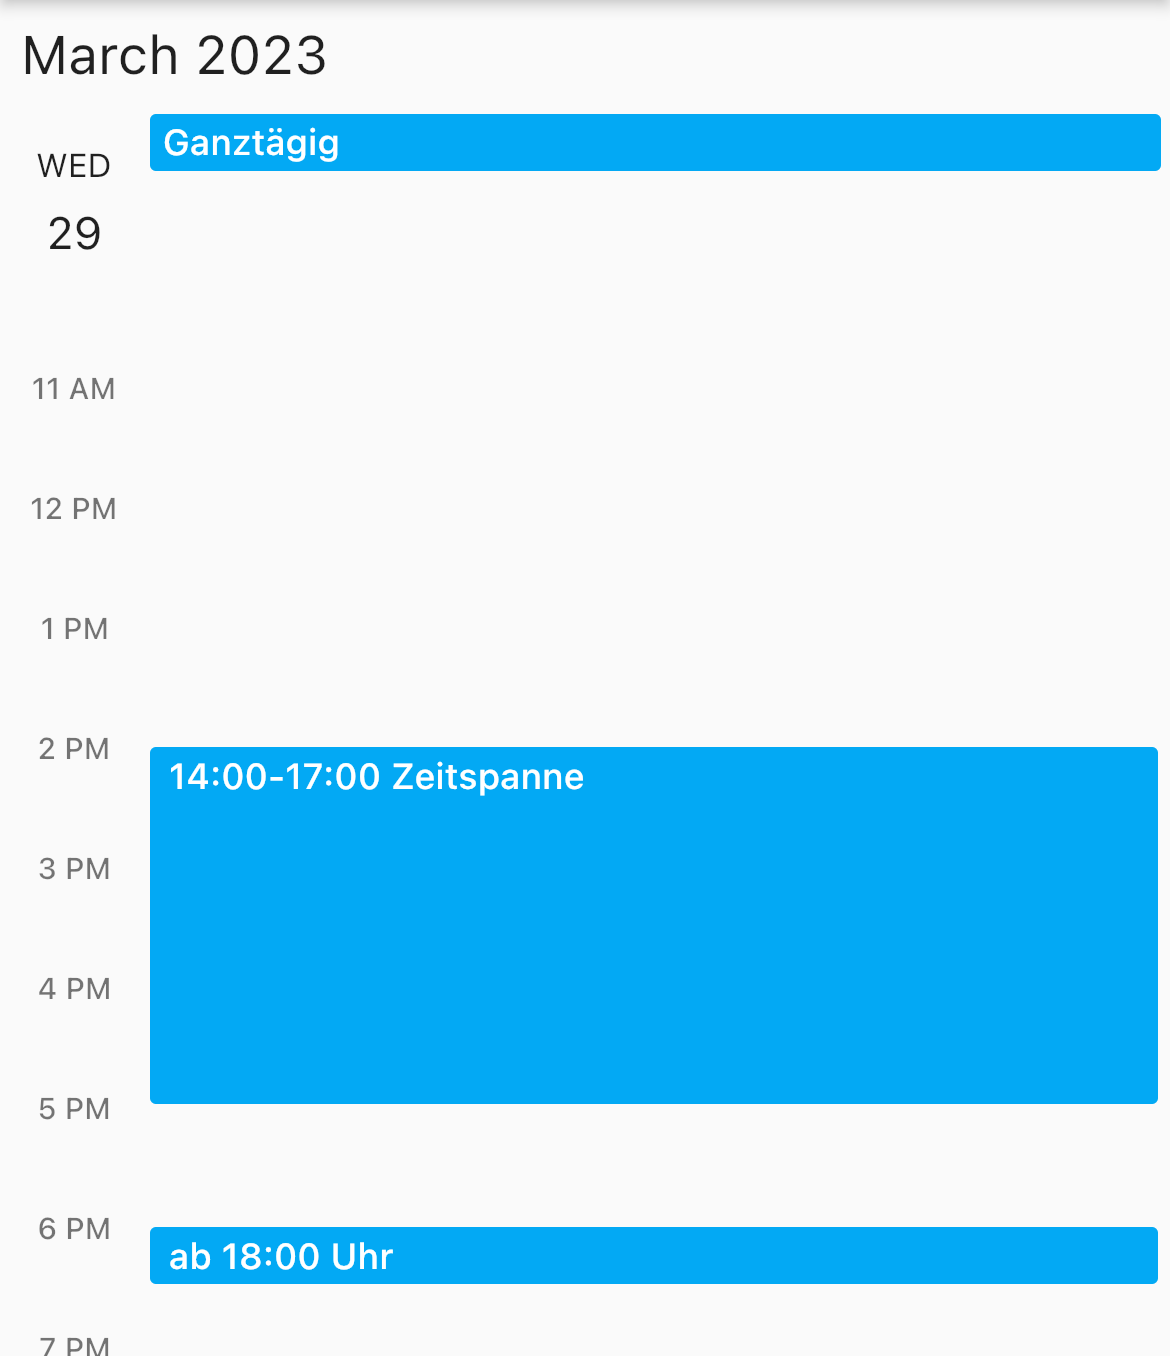
\includegraphics[width=0.6\textwidth]{res/zeitspanne.png} 
    \caption{Beispiel Darstellung einer Zeitangabe} 
    \label{pic:zeitspanne}
\end{figure}

%Fassade
\begin{figure}
    \centering
    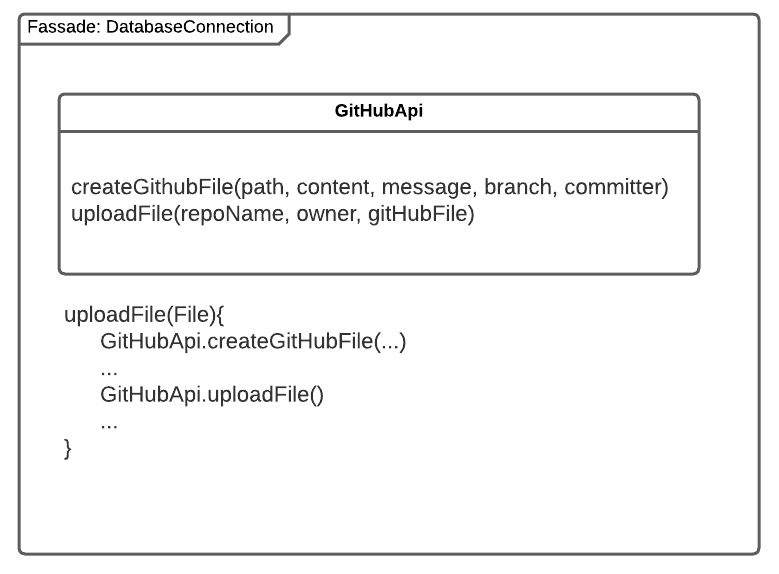
\includegraphics[width=0.9\textwidth]{res/fassade_database_connection.png} 
    \caption{Vereinfachte Darstellung der Fassade} 
    \label{pic:fassade_database_connection}
\end{figure}

%Singelton
\begin{figure}
    \centering
    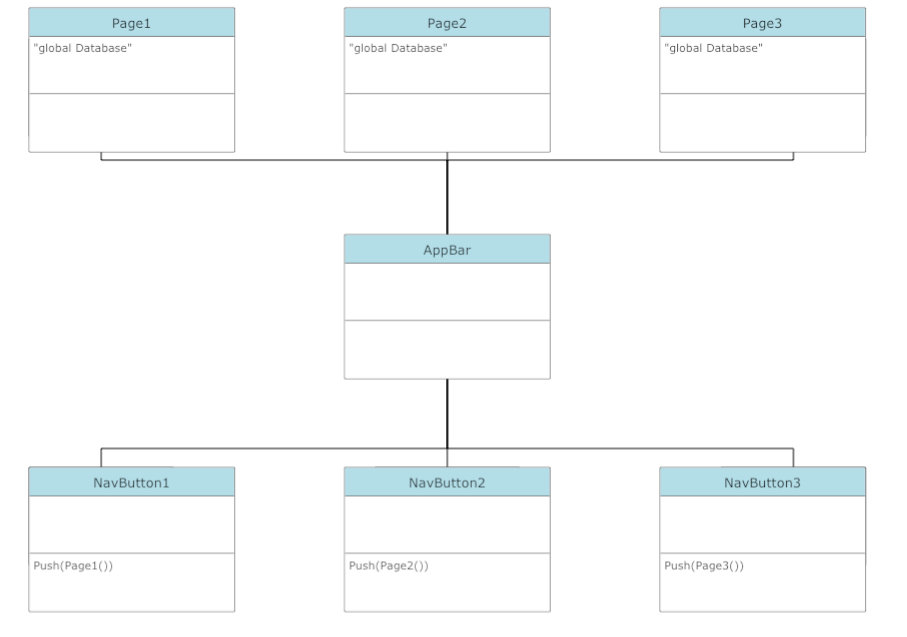
\includegraphics[width=1.1\textwidth]{res/global_database.png} 
    \caption{Globale Datenbank durch Singelton} 
    \label{pic:global_database}
\end{figure}
\begin{figure}
  \centering
  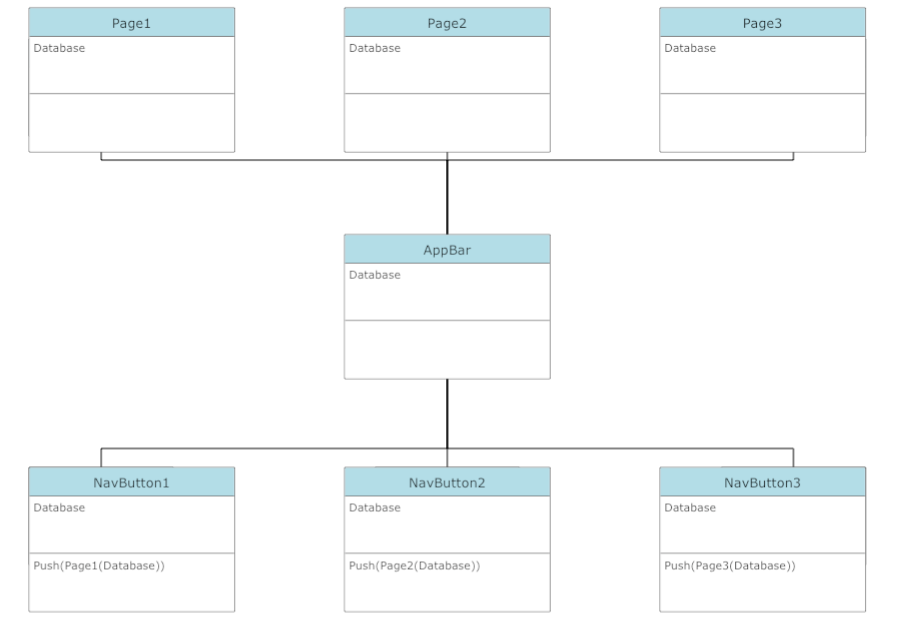
\includegraphics[width=1.1\linewidth]{res/weitergegebene_datasabe.png}
  \captionof{figure}{Weitergereichte Datenbank}
  \label{fig:weitergegebene_datasabe}
\end{figure}
\begin{figure}
  \centering
  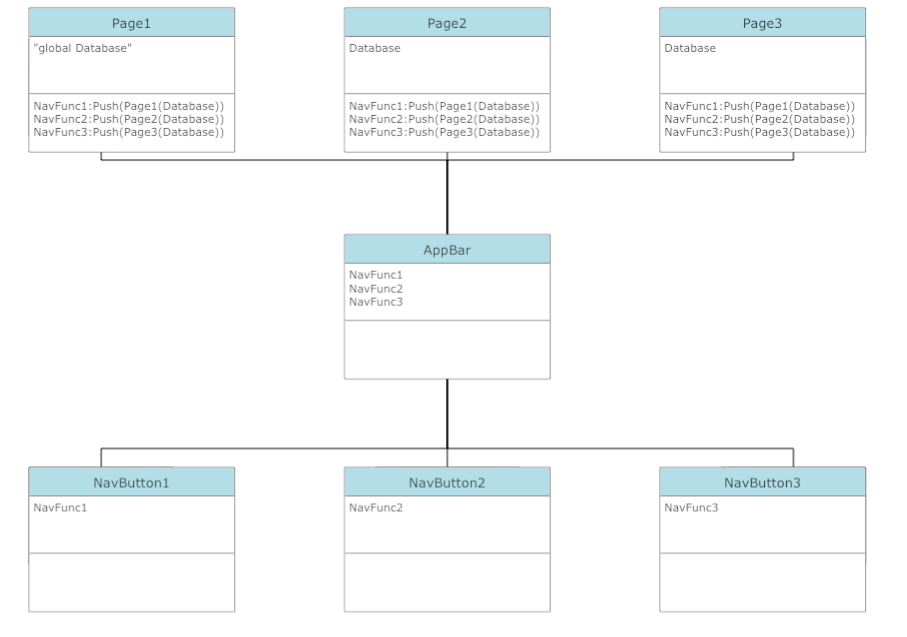
\includegraphics[width=1.1\linewidth]{res/hochgeschobene_nav_funktion.png}
  \captionof{figure}{Nach oben geschobene Navigationsfunktionen}
  \label{fig:hochgeschobene_nav_funktion}
\end{figure}


%Strategie
\begin{figure}
  \centering
  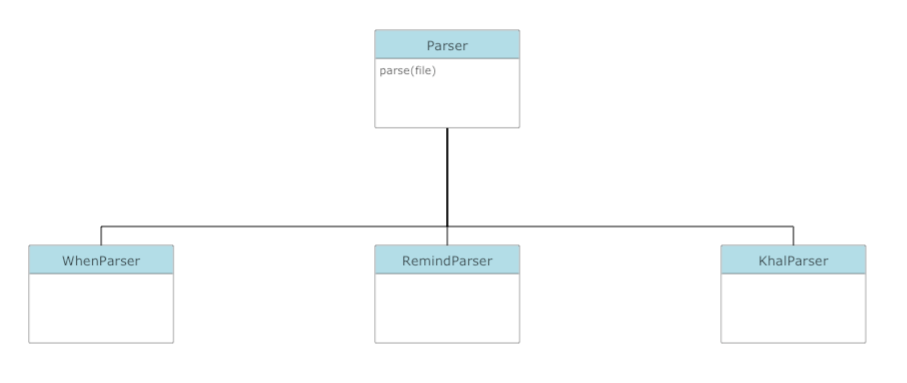
\includegraphics[width=1.1\linewidth]{res/strategie_parser.png}
  \captionof{figure}{Beispiel der Strategiedarstellung für den Parser}
  \label{fig:strategie_parser}
\end{figure}
\begin{figure}
  \centering
  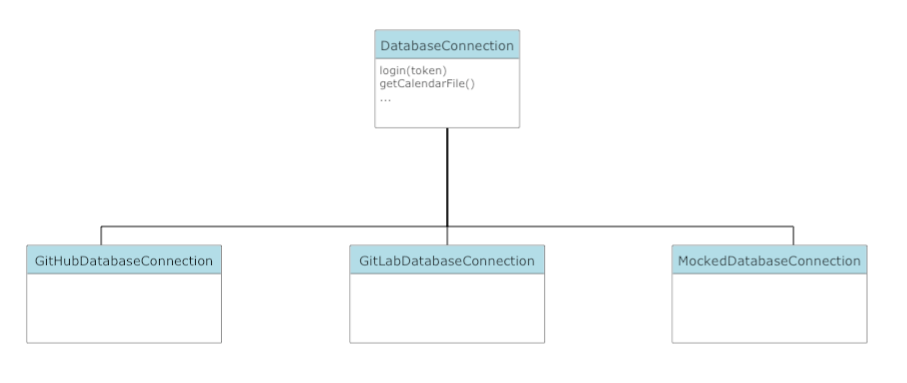
\includegraphics[width=1.1\linewidth]{res/strategie_database.png}
  \captionof{figure}{Beispiel der Strategiedarstellung für die Datenbank}
  \label{fig:strategie_database}
\end{figure}

%Proxy
\begin{figure}
    \centering
    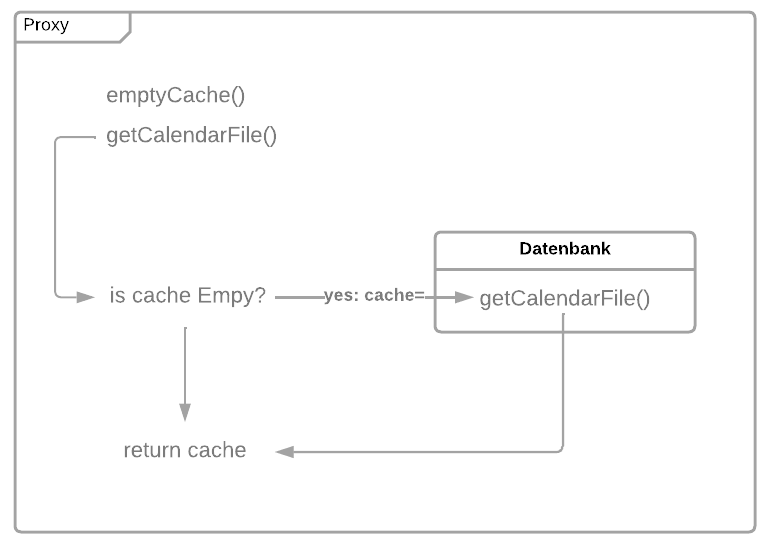
\includegraphics[width=0.8\textwidth]{res/proxy.png} 
    \caption{Vereinfachte Darstellung der Proxydatenbank} 
    \label{pic:proxy}
\end{figure}

%AblageBasiert
\begin{figure}
    \centering
    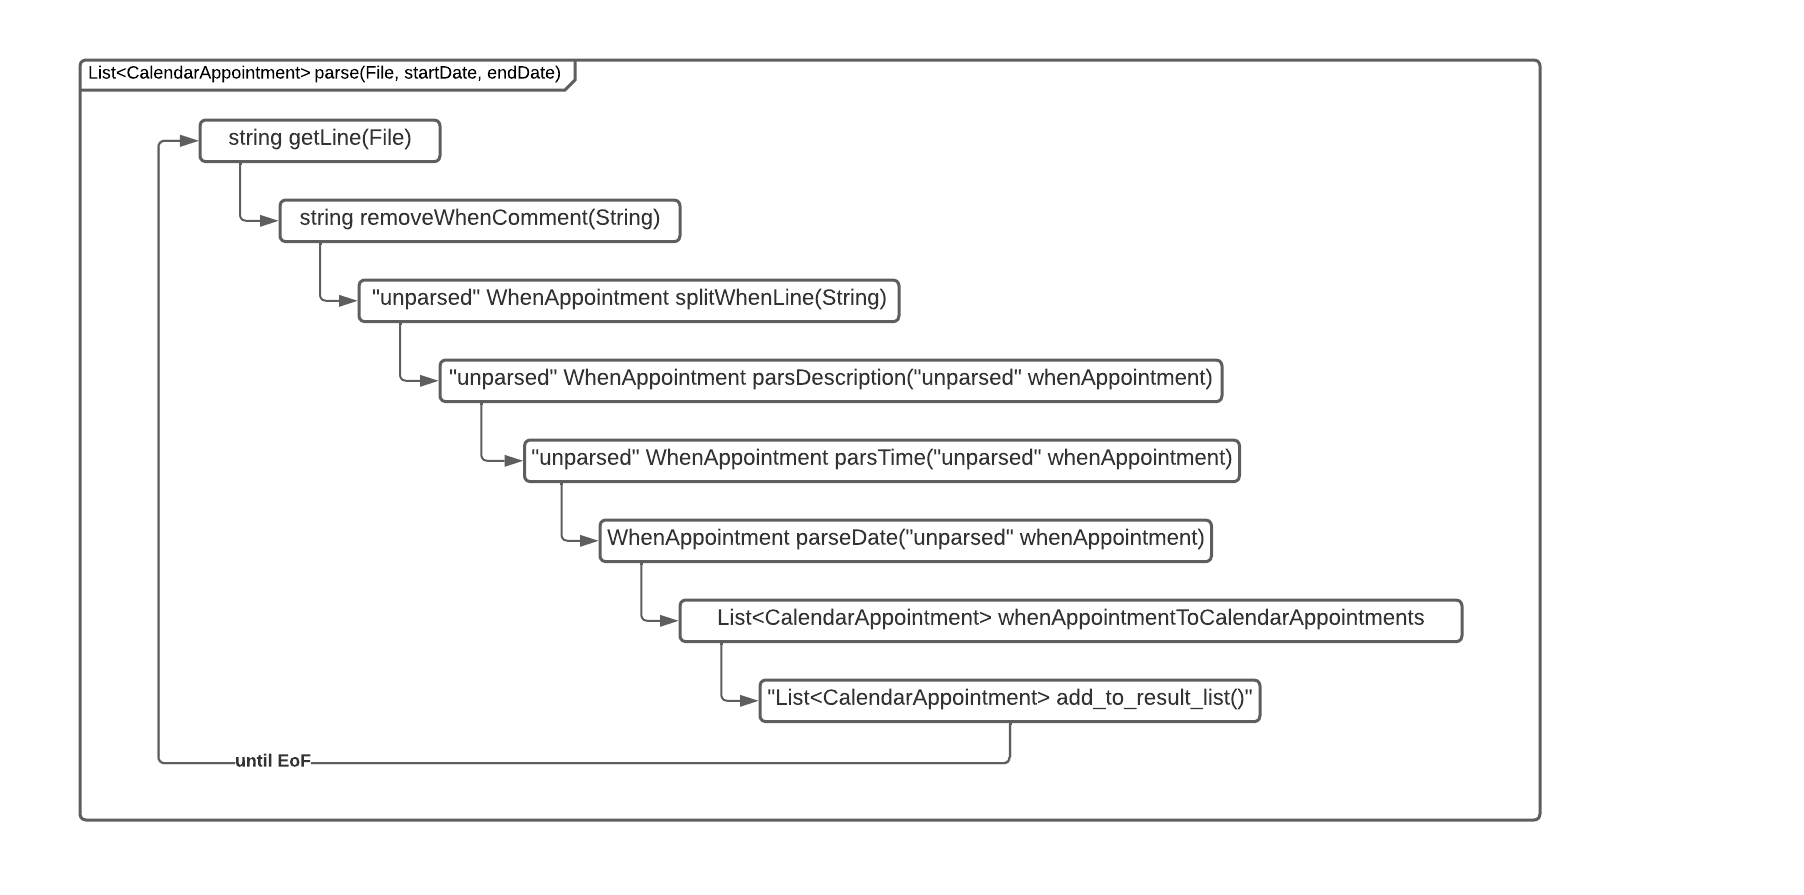
\includegraphics[width=1.2\textwidth]{res/datenfluss.png} 
    \caption{Ablauf mit der datenflussnetz ähnlichen Struktur} 
    \label{pic:datenfluss}
\end{figure}

\begin{figure}
  \centering
  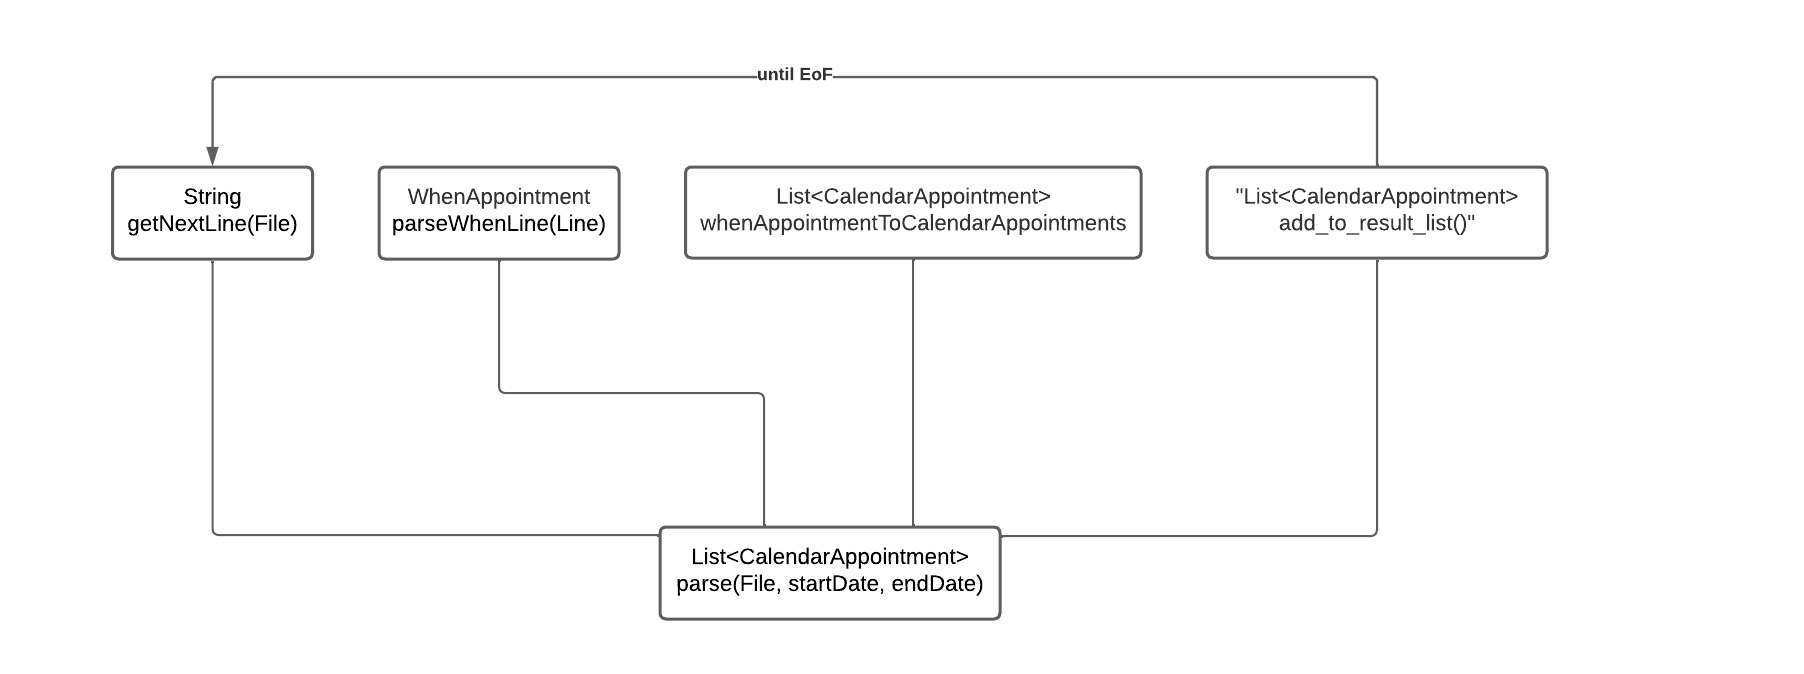
\includegraphics[width=1.2\linewidth]{res/Ablage-basiert1.png}
  \captionof{figure}{Ablauf mit der ablagebasierten ähnlichen Struktur Teil 1}
  \label{fig:ablage_basiert1}
\end{figure}
\begin{figure}
  \centering
  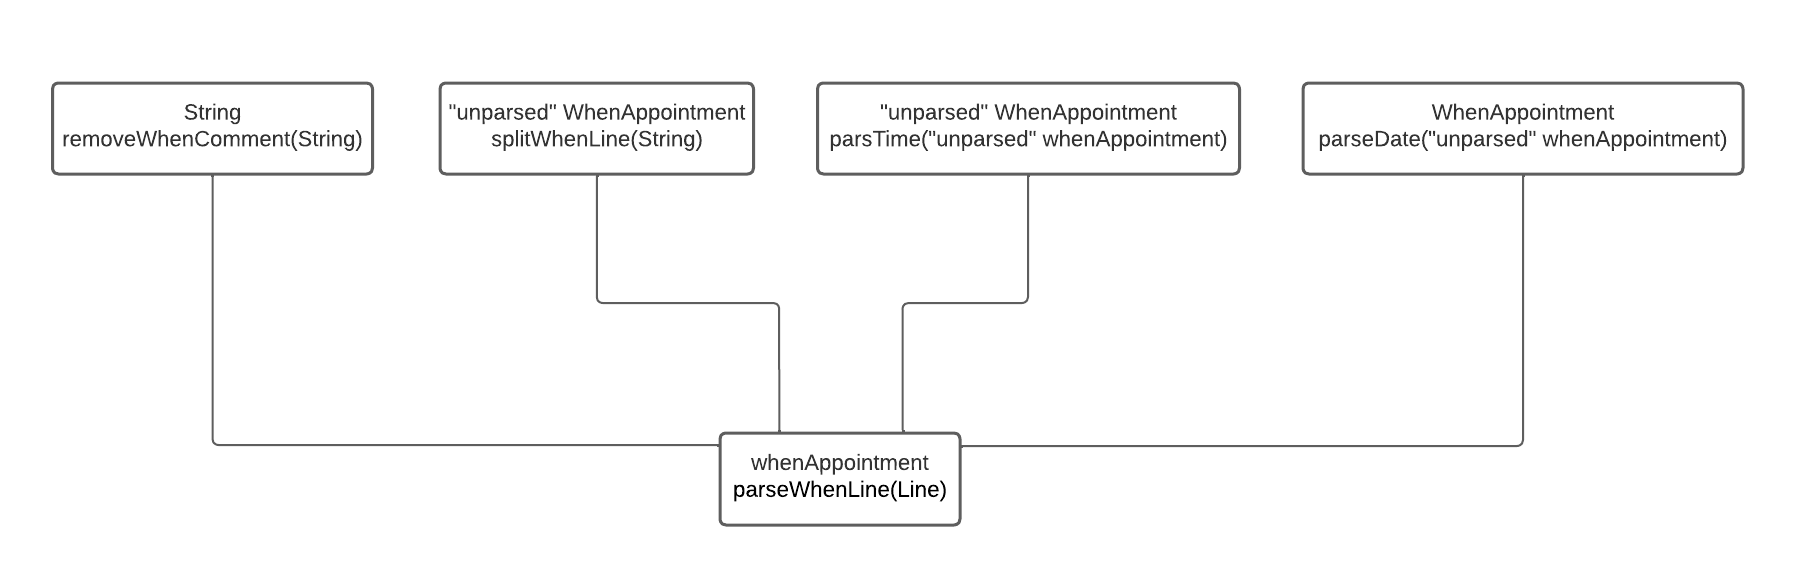
\includegraphics[width=1.2\linewidth]{res/Ablage-basiert2.png}
  \captionof{figure}{Ablauf mit der ablagebasierten ähnlichen Struktur Teil 2}
  \label{fig:ablage_basiert2}
\end{figure}
%



%reminders views comparison

\begin{figure}
    \centering
    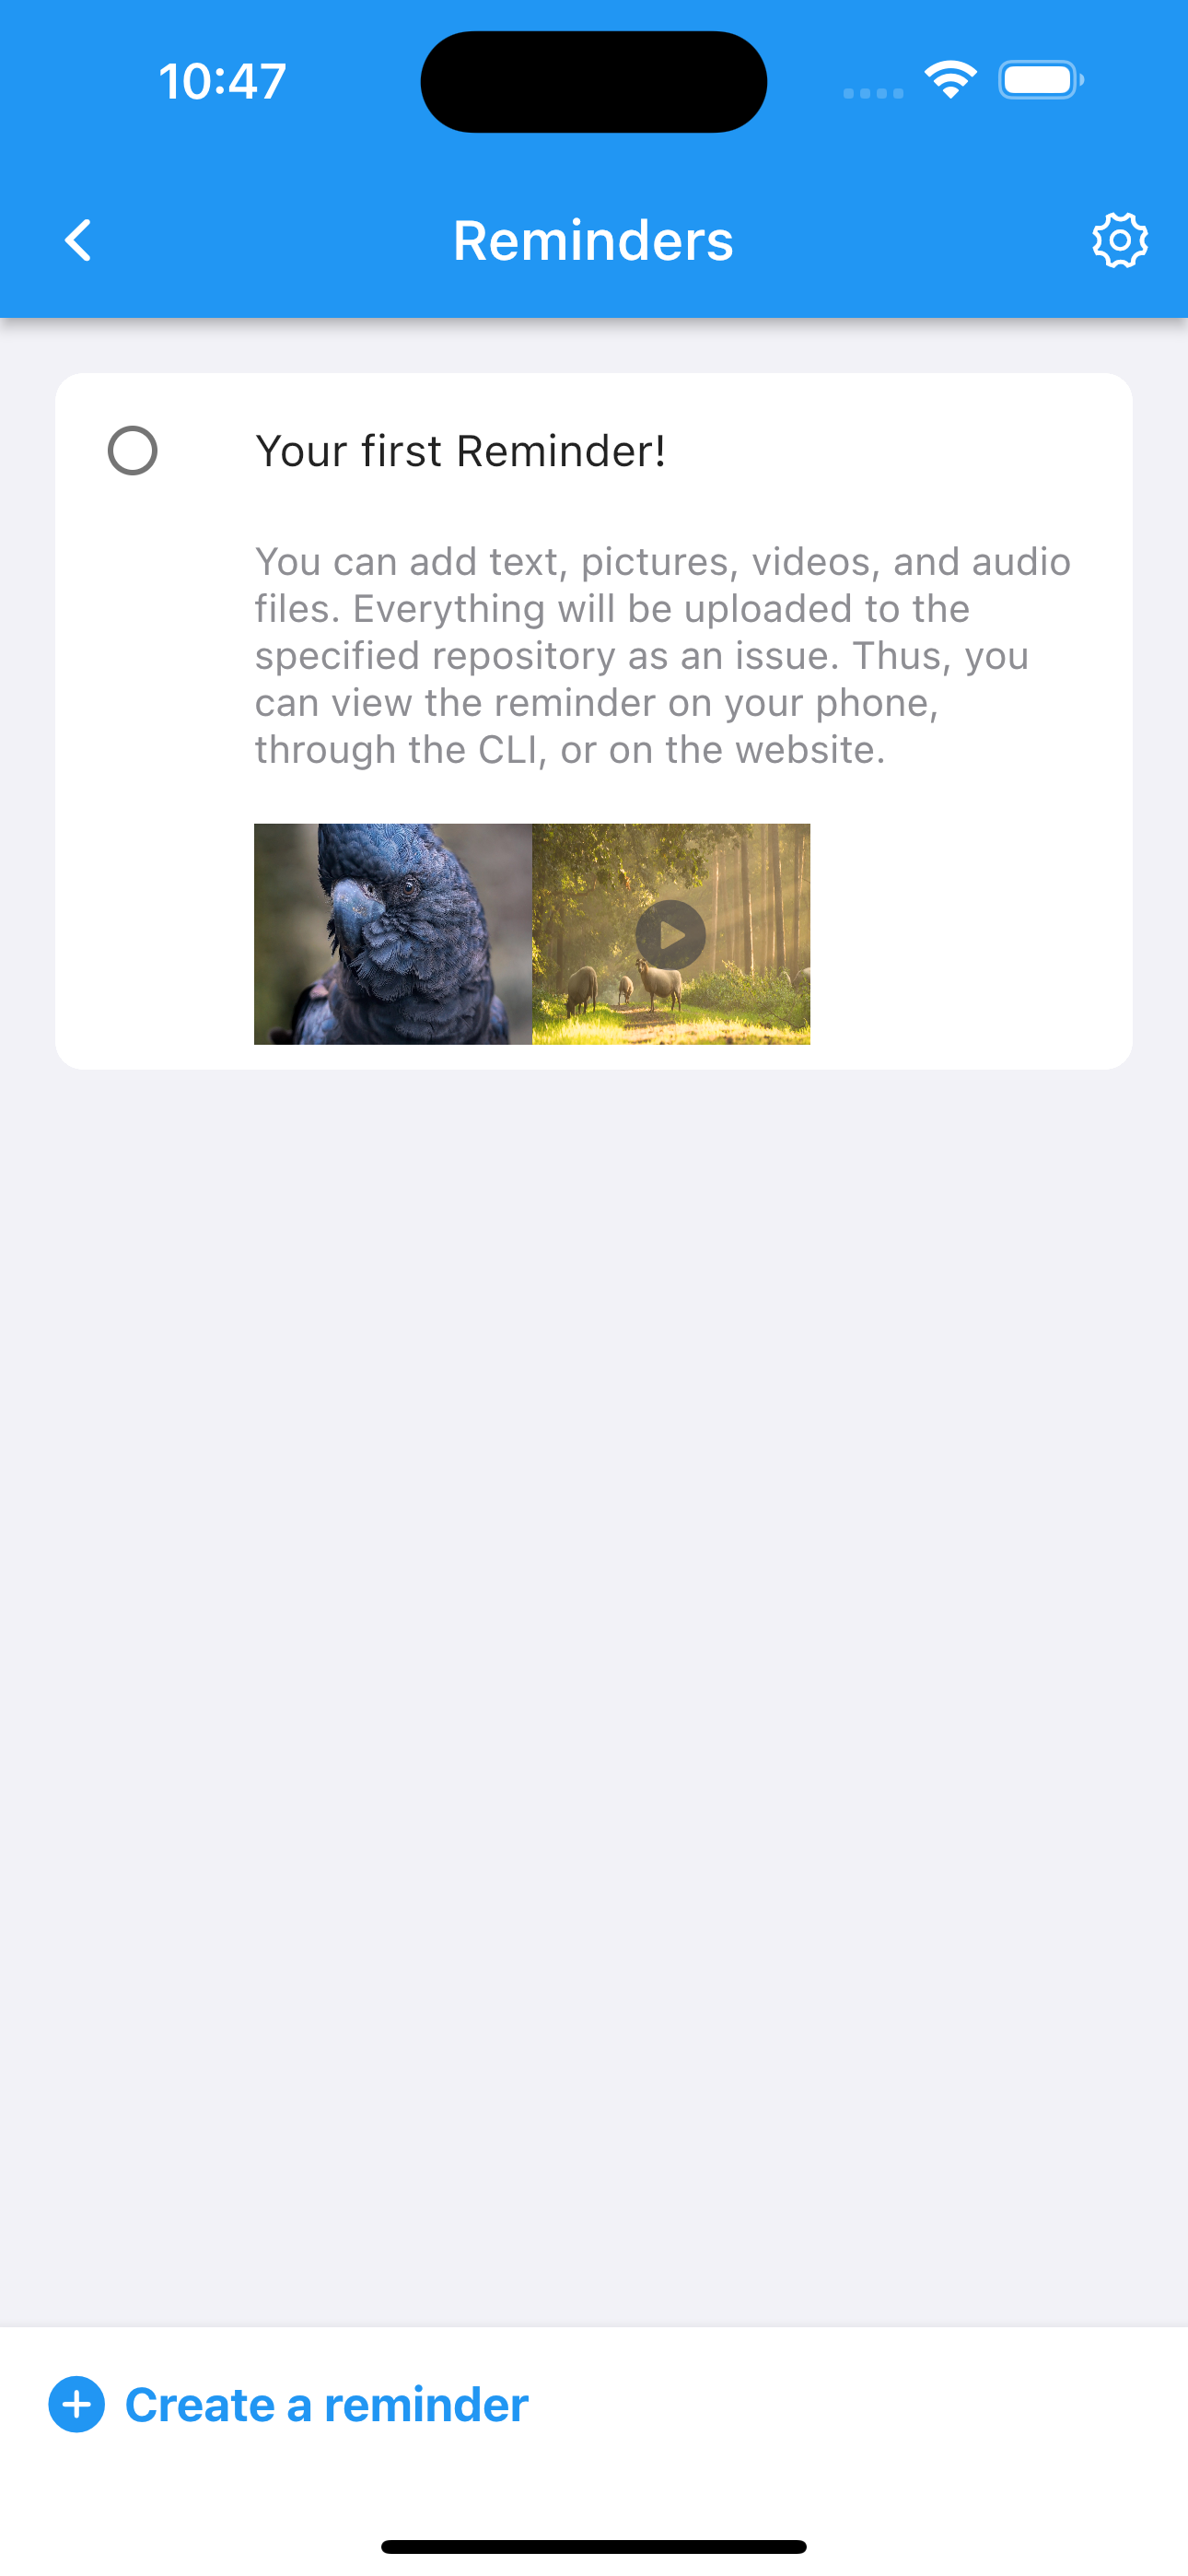
\includegraphics[width=.5\textwidth]{res/reminder_handy.png} 
    \caption{Handyansicht der Erinnerungen} 
    \label{pic:reminder_handy}
\end{figure}

\begin{figure}
    \centering
    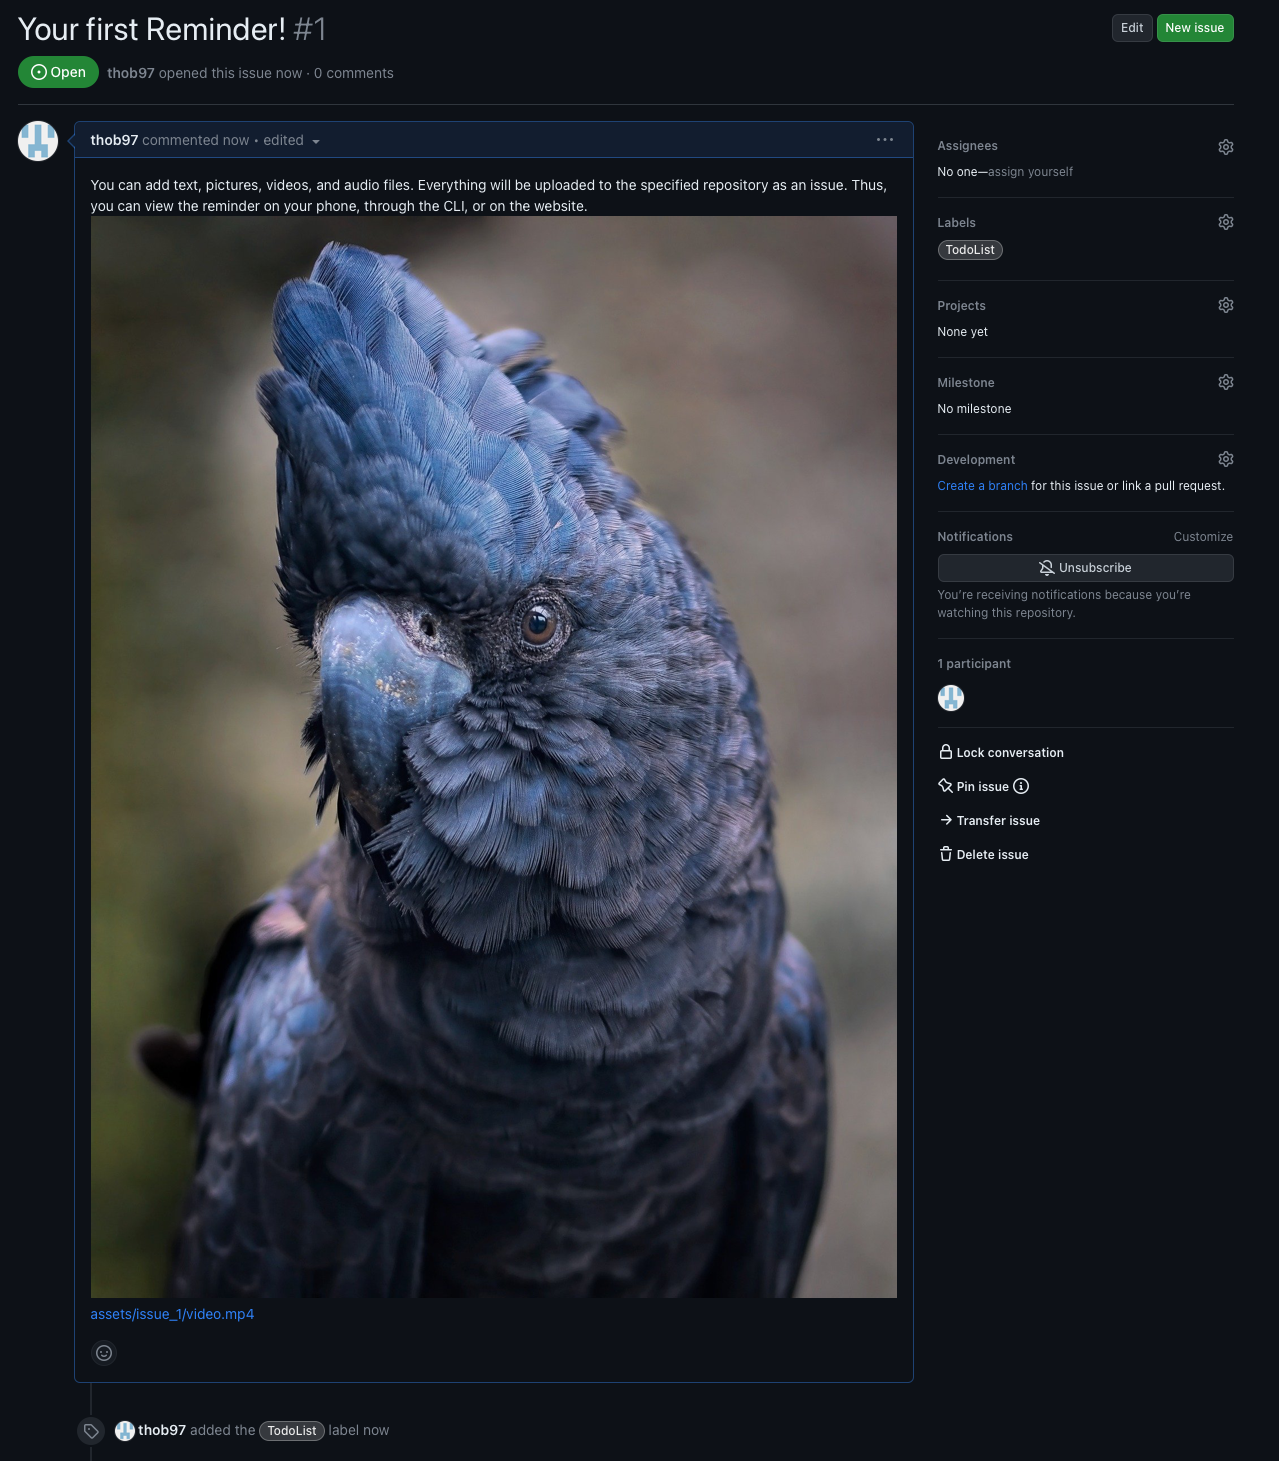
\includegraphics[width=1.1\textwidth]{res/reminders_webview.png} 
    \caption{Webseitenansicht der Erinnerungen} 
    \label{pic_webview}
\end{figure}

\begin{figure}
    \centering
    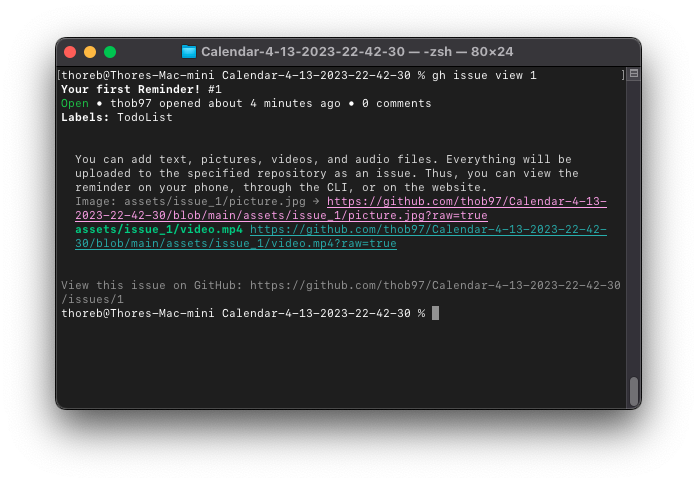
\includegraphics[width=1\textwidth]{res/reminder_cli.png} 
    \caption{CLI-Ansicht der Erinnerungen} 
    \label{pic_reminder_cli}
\end{figure}
